\documentclass{article}

\usepackage[utf8]{inputenc}
\usepackage{amsmath,amssymb,amsthm}
\usepackage{array}
\usepackage{enumitem}
\usepackage[left=3.5cm,right=3.5cm,top=2cm,bottom=2cm]{geometry}
\usepackage{graphicx}
\usepackage[vlined,ruled,norelsize,algo2e]{algorithm2e}

\title{Verified Path Following for Ackermann Car Model}
\author{Author}
\date{June 2022}

\theoremstyle{plain}
\newtheorem{lemma}{Lemma}
\newtheorem{theorem}{Theorem}
\newtheorem{proposition}{Proposition}
\newtheorem{corollary}{Corollary}
\theoremstyle{definition}
\newtheorem{definition}{Definition}
\newtheorem{assumption}{Assumption}
\newtheorem{problem}{Problem}
\theoremstyle{remark}
\newtheorem{remark}{Remark}
\newtheorem{example}{Example}

\newcommand{\calA}{\mathcal{A}}
\newcommand{\calB}{\mathcal{B}}
\newcommand{\calC}{\mathcal{C}}
\newcommand{\calD}{\mathcal{D}}
\newcommand{\calE}{\mathcal{E}}
\newcommand{\calF}{\mathcal{F}}
\newcommand{\calG}{\mathcal{G}}
\newcommand{\calH}{\mathcal{H}}
\newcommand{\calI}{\mathcal{I}}
\newcommand{\calJ}{\mathcal{J}}
\newcommand{\calK}{\mathcal{K}}
\newcommand{\calL}{\mathcal{L}}
\newcommand{\calM}{\mathcal{M}}
\newcommand{\calN}{\mathcal{N}}
\newcommand{\calO}{\mathcal{O}}
\newcommand{\calP}{\mathcal{P}}
\newcommand{\calQ}{\mathcal{Q}}
\newcommand{\calR}{\mathcal{R}}
\newcommand{\calS}{\mathcal{S}}
\newcommand{\calT}{\mathcal{T}}
\newcommand{\calU}{\mathcal{U}}
\newcommand{\calV}{\mathcal{V}}
\newcommand{\calW}{\mathcal{W}}
\newcommand{\calX}{\mathcal{X}}
\newcommand{\calY}{\mathcal{Y}}
\newcommand{\calZ}{\mathcal{Z}}

\newcommand{\Ahat}{\hat{A}}
\newcommand{\Bhat}{\hat{B}}
\newcommand{\Chat}{\hat{C}}
\newcommand{\Dhat}{\hat{D}}
\newcommand{\Ehat}{\hat{E}}
\newcommand{\Fhat}{\hat{F}}
\newcommand{\Ghat}{\hat{G}}
\newcommand{\Hhat}{\hat{H}}
\newcommand{\Ihat}{\hat{I}}
\newcommand{\Jhat}{\hat{J}}
\newcommand{\Khat}{\hat{K}}
\newcommand{\Lhat}{\hat{L}}
\newcommand{\Mhat}{\hat{M}}
\newcommand{\Nhat}{\hat{N}}
\newcommand{\Ohat}{\hat{O}}
\newcommand{\Phat}{\hat{P}}
\newcommand{\Qhat}{\hat{Q}}
\newcommand{\Rhat}{\hat{R}}
\newcommand{\Shat}{\hat{S}}
\newcommand{\That}{\hat{T}}
\newcommand{\Uhat}{\hat{U}}
\newcommand{\Vhat}{\hat{V}}
\newcommand{\What}{\hat{W}}
\newcommand{\Xhat}{\hat{X}}
\newcommand{\Yhat}{\hat{Y}}
\newcommand{\Zhat}{\hat{Z}}

\newcommand{\ahat}{\hat{a}}
\newcommand{\bhat}{\hat{b}}
\newcommand{\chat}{\hat{c}}
\newcommand{\dhat}{\hat{d}}
\newcommand{\ehat}{\hat{e}}
\newcommand{\fhat}{\hat{f}}
\newcommand{\ghat}{\hat{g}}
\newcommand{\hhat}{\hat{h}}
\newcommand{\ihat}{\hat{i}}
\newcommand{\jhat}{\hat{j}}
\newcommand{\khat}{\hat{k}}
\newcommand{\lhat}{\hat{l}}
\newcommand{\mhat}{\hat{m}}
\newcommand{\nhat}{\hat{n}}
\newcommand{\ohat}{\hat{o}}
\newcommand{\phat}{\hat{p}}
\newcommand{\qhat}{\hat{q}}
\newcommand{\rhat}{\hat{r}}
\newcommand{\shat}{\hat{s}}
\newcommand{\that}{\hat{t}}
\newcommand{\uhat}{\hat{u}}
\newcommand{\vhat}{\hat{v}}
\newcommand{\what}{\hat{w}}
\newcommand{\xhat}{\hat{x}}
\newcommand{\yhat}{\hat{y}}
\newcommand{\zhat}{\hat{z}}

\newcommand{\sigmahat}{\hat\sigma}
\newcommand{\phihat}{\hat\phi}
\newcommand{\gammahat}{\hat\gamma}
\newcommand{\xihat}{\hat\xi}
\newcommand{\Xihat}{\hat\Xi}
\newcommand{\epsilonhat}{\hat\epsilon}
\newcommand{\Sigmahat}{\hat\Sigma}
\newcommand{\Omegahat}{\hat\Omega}

\newcommand{\Abar}{\bar{A}}
\newcommand{\Bbar}{\bar{B}}
\newcommand{\Cbar}{\bar{C}}
\newcommand{\Dbar}{\bar{D}}
\newcommand{\Ebar}{\bar{E}}
\newcommand{\Fbar}{\bar{F}}
\newcommand{\Gbar}{\bar{G}}
\newcommand{\Hbar}{\bar{H}}
\newcommand{\Ibar}{\bar{I}}
\newcommand{\Jbar}{\bar{J}}
\newcommand{\Kbar}{\bar{K}}
\newcommand{\Lbar}{\bar{L}}
\newcommand{\Mbar}{\bar{M}}
\newcommand{\Nbar}{\bar{N}}
\newcommand{\Obar}{\bar{O}}
\newcommand{\Pbar}{\bar{P}}
\newcommand{\Qbar}{\bar{Q}}
\newcommand{\Rbar}{\bar{R}}
\newcommand{\Sbar}{\bar{S}}
\newcommand{\Tbar}{\bar{T}}
\newcommand{\Ubar}{\bar{U}}
\newcommand{\Vbar}{\bar{V}}
\newcommand{\Wbar}{\bar{W}}
\newcommand{\Xbar}{\bar{X}}
\newcommand{\Ybar}{\bar{Y}}
% \newcommand{\Zbar}{\bar{Z}}

\newcommand{\abar}{\bar{a}}
\newcommand{\bbar}{\bar{b}}
\newcommand{\cbar}{\bar{c}}
\newcommand{\dbar}{\bar{d}}
\newcommand{\ebar}{\bar{e}}
\newcommand{\fbar}{\bar{f}}
\newcommand{\gbar}{\bar{g}}
% \newcommand{\hbar}{\bar{h}}
\newcommand{\ibar}{\bar{i}}
\newcommand{\jbar}{\bar{j}}
\newcommand{\kbar}{\bar{k}}
\newcommand{\lbar}{\bar{l}}
\newcommand{\mbar}{\bar{m}}
\newcommand{\nbar}{\bar{n}}
% \newcommand{\obar}{\bar{o}}
\newcommand{\pbar}{\bar{p}}
\newcommand{\qbar}{\bar{q}}
\newcommand{\rbar}{\bar{r}}
\newcommand{\sbar}{\bar{s}}
\newcommand{\tbar}{\bar{t}}
\newcommand{\ubar}{\bar{u}}
\newcommand{\vbar}{\bar{v}}
\newcommand{\wbar}{\bar{w}}
\newcommand{\xbar}{\bar{x}}
\newcommand{\ybar}{\bar{y}}
\newcommand{\zbar}{\bar{z}}

\newcommand{\alphabar}{\bar{\alpha}}
\newcommand{\gammabar}{\bar{\gamma}}
\newcommand{\varepsilonbar}{\bar{\varepsilon}}
\newcommand{\epsilonbar}{\bar{\epsilon}}
\newcommand{\thetabar}{\bar{\theta}}
\newcommand{\sigmabar}{\bar{\sigma}}
\newcommand{\mubar}{\bar{\mu}}
\newcommand{\nubar}{\bar{\nu}}
\newcommand{\omegabar}{\bar{\omega}}
\newcommand{\Omegabar}{\bar{\Omega}}

\newcommand{\Atilde}{\tilde{A}}
\newcommand{\Btilde}{\tilde{B}}
\newcommand{\Ctilde}{\tilde{C}}
\newcommand{\Dtilde}{\tilde{D}}
\newcommand{\Etilde}{\tilde{E}}
\newcommand{\Ftilde}{\tilde{F}}
\newcommand{\Gtilde}{\tilde{G}}
\newcommand{\Htilde}{\tilde{H}}
\newcommand{\Itilde}{\tilde{I}}
\newcommand{\Jtilde}{\tilde{J}}
\newcommand{\Ktilde}{\tilde{K}}
\newcommand{\Ltilde}{\tilde{L}}
\newcommand{\Mtilde}{\tilde{M}}
\newcommand{\Ntilde}{\tilde{N}}
\newcommand{\Otilde}{\tilde{O}}
\newcommand{\Ptilde}{\tilde{P}}
\newcommand{\Qtilde}{\tilde{Q}}
\newcommand{\Rtilde}{\tilde{R}}
\newcommand{\Stilde}{\tilde{S}}
\newcommand{\Ttilde}{\tilde{T}}
\newcommand{\Utilde}{\tilde{U}}
\newcommand{\Vtilde}{\tilde{V}}
\newcommand{\Wtilde}{\tilde{W}}
\newcommand{\Xtilde}{\tilde{X}}
\newcommand{\Ytilde}{\tilde{Y}}
\newcommand{\Ztilde}{\tilde{Z}}

\newcommand{\atilde}{\tilde{a}}
\newcommand{\btilde}{\tilde{b}}
\newcommand{\ctilde}{\tilde{c}}
\newcommand{\dtilde}{\tilde{d}}
\newcommand{\etilde}{\tilde{e}}
\newcommand{\ftilde}{\tilde{f}}
\newcommand{\gtilde}{\tilde{g}}
\newcommand{\htilde}{\tilde{h}}
\newcommand{\itilde}{\tilde{i}}
\newcommand{\jtilde}{\tilde{j}}
\newcommand{\ktilde}{\tilde{k}}
\newcommand{\ltilde}{\tilde{l}}
\newcommand{\mtilde}{\tilde{m}}
\newcommand{\ntilde}{\tilde{n}}
\newcommand{\otilde}{\tilde{o}}
\newcommand{\ptilde}{\tilde{p}}
\newcommand{\qtilde}{\tilde{q}}
\newcommand{\rtilde}{\tilde{r}}
\newcommand{\stilde}{\tilde{s}}
\newcommand{\ttilde}{\tilde{t}}
\newcommand{\utilde}{\tilde{u}}
\newcommand{\vtilde}{\tilde{v}}
\newcommand{\wtilde}{\tilde{w}}
\newcommand{\xtilde}{\tilde{x}}
\newcommand{\ytilde}{\tilde{y}}
\newcommand{\ztilde}{\tilde{z}}

\newcommand{\gammatilde}{\tilde{\gamma}}
\newcommand{\zetatilde}{\tilde{\zeta}}
\newcommand{\thetatilde}{\tilde{\theta}}
\newcommand{\omegatilde}{\tilde{\omega}}
\newcommand{\Sigmatilde}{\tilde{\Sigma}}
\newcommand{\Omegatilde}{\tilde{\Omega}}

\newcommand{\arm}{\mathrm{a}}
\newcommand{\brm}{\mathrm{b}}
\newcommand{\crm}{\mathrm{c}}
\newcommand{\drm}{\mathrm{d}}
\newcommand{\erm}{\mathrm{e}}
\newcommand{\frm}{\mathrm{f}}
\newcommand{\grm}{\mathrm{g}}
\newcommand{\hrm}{\mathrm{h}}
\newcommand{\irm}{\mathrm{i}}
\newcommand{\jrm}{\mathrm{j}}
\newcommand{\krm}{\mathrm{k}}
\newcommand{\lrm}{\mathrm{l}}
\newcommand{\mrm}{\mathrm{m}}
\newcommand{\nrm}{\mathrm{n}}
\newcommand{\orm}{\mathrm{o}}
\newcommand{\prm}{\mathrm{p}}
\newcommand{\qrm}{\mathrm{q}}
\newcommand{\rrm}{\mathrm{r}}
\newcommand{\srm}{\mathrm{s}}
\newcommand{\trm}{\mathrm{t}}
\newcommand{\urm}{\mathrm{u}}
\newcommand{\vrm}{\mathrm{v}}
\newcommand{\wrm}{\mathrm{w}}
\newcommand{\xrm}{\mathrm{x}}
\newcommand{\yrm}{\mathrm{y}}
\newcommand{\zrm}{\mathrm{z}}

\newcommand{\Arm}{\mathrm{A}}
\newcommand{\Brm}{\mathrm{B}}
\newcommand{\Crm}{\mathrm{C}}
\newcommand{\Drm}{\mathrm{D}}
\newcommand{\Erm}{\mathrm{E}}
\newcommand{\Frm}{\mathrm{F}}
\newcommand{\Grm}{\mathrm{G}}
\newcommand{\Hrm}{\mathrm{H}}
\newcommand{\Irm}{\mathrm{I}}
\newcommand{\Jrm}{\mathrm{J}}
\newcommand{\Krm}{\mathrm{K}}
\newcommand{\Lrm}{\mathrm{L}}
\newcommand{\Mrm}{\mathrm{M}}
\newcommand{\Nrm}{\mathrm{N}}
\newcommand{\Orm}{\mathrm{O}}
\newcommand{\Prm}{\mathrm{P}}
\newcommand{\Qrm}{\mathrm{Q}}
\newcommand{\Rrm}{\mathrm{R}}
\newcommand{\Srm}{\mathrm{S}}
\newcommand{\Trm}{\mathrm{T}}
\newcommand{\Urm}{\mathrm{U}}
\newcommand{\Vrm}{\mathrm{V}}
\newcommand{\Wrm}{\mathrm{W}}
\newcommand{\Xrm}{\mathrm{X}}
\newcommand{\Yrm}{\mathrm{Y}}
\newcommand{\Zrm}{\mathrm{Z}}

\newcommand{\afrak}{\mathfrak{a}}
\newcommand{\bfrak}{\mathfrak{b}}
\newcommand{\cfrak}{\mathfrak{c}}
\newcommand{\dfrak}{\mathfrak{d}}
\newcommand{\efrak}{\mathfrak{e}}
\newcommand{\ffrak}{\mathfrak{f}}
\newcommand{\gfrak}{\mathfrak{g}}
\newcommand{\hfrak}{\mathfrak{h}}
\newcommand{\ifrak}{\mathfrak{i}}
\newcommand{\jfrak}{\mathfrak{j}}
\newcommand{\kfrak}{\mathfrak{k}}
\newcommand{\lfrak}{\mathfrak{l}}
\newcommand{\mfrak}{\mathfrak{m}}
\newcommand{\nfrak}{\mathfrak{n}}
\newcommand{\ofrak}{\mathfrak{o}}
\newcommand{\pfrak}{\mathfrak{p}}
\newcommand{\qfrak}{\mathfrak{q}}
\newcommand{\rfrak}{\mathfrak{r}}
\newcommand{\sfrak}{\mathfrak{s}}
\newcommand{\tfrak}{\mathfrak{t}}
\newcommand{\ufrak}{\mathfrak{u}}
\newcommand{\vfrak}{\mathfrak{v}}
\newcommand{\wfrak}{\mathfrak{w}}
\newcommand{\xfrak}{\mathfrak{x}}
\newcommand{\yfrak}{\mathfrak{y}}
\newcommand{\zfrak}{\mathfrak{z}}

\newcommand{\Afrak}{\mathfrak{A}}
\newcommand{\Bfrak}{\mathfrak{B}}
\newcommand{\Cfrak}{\mathfrak{C}}
\newcommand{\Dfrak}{\mathfrak{D}}
\newcommand{\Efrak}{\mathfrak{E}}
\newcommand{\Ffrak}{\mathfrak{F}}
\newcommand{\Gfrak}{\mathfrak{G}}
\newcommand{\Hfrak}{\mathfrak{H}}
\newcommand{\Ifrak}{\mathfrak{I}}
\newcommand{\Jfrak}{\mathfrak{J}}
\newcommand{\Kfrak}{\mathfrak{K}}
\newcommand{\Lfrak}{\mathfrak{L}}
\newcommand{\Mfrak}{\mathfrak{M}}
\newcommand{\Nfrak}{\mathfrak{N}}
\newcommand{\Ofrak}{\mathfrak{O}}
\newcommand{\Pfrak}{\mathfrak{P}}
\newcommand{\Qfrak}{\mathfrak{Q}}
\newcommand{\Rfrak}{\mathfrak{R}}
\newcommand{\Sfrak}{\mathfrak{S}}
\newcommand{\Tfrak}{\mathfrak{T}}
\newcommand{\Ufrak}{\mathfrak{U}}
\newcommand{\Vfrak}{\mathfrak{V}}
\newcommand{\Wfrak}{\mathfrak{W}}
\newcommand{\Xfrak}{\mathfrak{X}}
\newcommand{\Yfrak}{\mathfrak{Y}}
\newcommand{\Zfrak}{\mathfrak{Z}}

\newcommand{\tta}{\mathtt{a}}
\newcommand{\ttb}{\mathtt{b}}
\newcommand{\ttc}{\mathtt{c}}
\newcommand{\ttd}{\mathtt{d}}
\newcommand{\tte}{\mathtt{e}}
\newcommand{\ttf}{\mathtt{f}}
\newcommand{\ttg}{\mathtt{g}}
\newcommand{\tth}{\mathtt{h}}
\newcommand{\tti}{\mathtt{i}}
\newcommand{\ttj}{\mathtt{j}}
\newcommand{\ttk}{\mathtt{k}}
\newcommand{\ttl}{\mathtt{l}}
\newcommand{\ttm}{\mathtt{m}}
\newcommand{\ttn}{\mathtt{n}}
\newcommand{\tto}{\mathtt{o}}
\newcommand{\ttp}{\mathtt{p}}
\newcommand{\ttq}{\mathtt{q}}
\newcommand{\ttr}{\mathtt{r}}
\newcommand{\tts}{\mathtt{s}}
\newcommand{\ttt}{\mathtt{t}}
\newcommand{\ttu}{\mathtt{u}}
\newcommand{\ttv}{\mathtt{v}}
\newcommand{\ttw}{\mathtt{w}}
\newcommand{\ttx}{\mathtt{x}}
\newcommand{\tty}{\mathtt{y}}
\newcommand{\ttz}{\mathtt{z}}

\renewcommand{\Re}{\mathbb{R}}
\newcommand{\Co}{\mathbb{C}}
\newcommand{\Ne}{\mathbb{N}}
\newcommand{\Ze}{\mathbb{Z}}
\newcommand{\saufzero}{\setminus\{0\}}
\newcommand{\nxn}{{n\times n}}
\newcommand{\mxn}{{m\times n}}
\newcommand{\nxm}{{n\times m}}
\newcommand{\dxd}{{d\times d}}
\newcommand{\exd}{{e\times d}}
\newcommand{\dxe}{{d\times e}}
\newcommand{\nint}{\mathrm{int}}
\newcommand{\bd}{\mathrm{bd}}
\newcommand{\dom}{\mathrm{dom}}
\newcommand{\diff}{\mathrm{d}}
\newcommand{\realp}{\mathrm{Re}}
\newcommand{\imagp}{\mathrm{Im}}
\newcommand{\conv}{\mathrm{conv}}
\newcommand{\rank}{\mathrm{rank}}
\newcommand{\diag}{\mathrm{diag}}
\newcommand{\trace}{\mathrm{trace}}
\newcommand{\vol}{\mathrm{vol}}
\newcommand{\mintxt}{\mathrm{min}}
\newcommand{\maxtxt}{\mathrm{max}}
\newcommand{\argmin}{\mathrm{arg\,min}}
\newcommand{\argmax}{\mathrm{arg\,max}}
\newcommand{\Ker}{\mathrm{Ker}}
\newcommand{\spann}{\mathrm{span}}
\newcommand{\dime}{\mathrm{dim}}
\newcommand{\Imag}{\mathrm{Im}}
\newcommand{\Prob}{\mathbb{P}}
\newcommand{\SSb}{\mathbb{S}}
\newcommand{\BBb}{\mathbb{B}}
\newcommand{\sign}{\mathrm{sign}}
\newcommand{\vecc}{\mathrm{vec}}
\newcommand{\specc}{\mathrm{spec}}

\newcommand{\comgb}[1]{{\upshape\footnotesize\texttt{[[}GB:{\sffamily\upshape\color{purple}~#1}\texttt{]]}}}
\newcommand{\new}{\color{blue}}
\newcommand{\newgb}{\color{red}}

\newcommand{\smax}{s_\maxtxt}
\newcommand{\sopt}{s_{\mathrm{opt}}}
\newcommand{\deltamax}{\delta_\maxtxt}
\newcommand{\alphamax}{\alpha_\maxtxt}
\newcommand{\rhoreq}{\rho_{\mathrm{req}}}
\newcommand{\calIreq}{\calI_{\mathrm{req}}}
\newcommand{\sreq}{s_{\mathrm{req}}}
\newcommand{\gammareq}{\gamma_{\mathrm{req}}}
\newcommand{\deltareq}{\delta_{\mathrm{req}}}
\newcommand{\alphareq}{\alpha_{\mathrm{req}}}

\begin{document}

\maketitle

\begin{abstract}
Sections~\ref{sec-introduction} to~\ref{sec-curved} are reminders of stuffs
that are present in the CoRL paper and stuffs that we discussed during meetings,
about extending straight path following CLF to curved and nonsmooth path following CLFs.
The novelty is in Section~\ref{sec-computation} which presents an algorithmic framework to compute
straight path following CLFs with prescribed properties.
Section~\ref{sec-simulation} demonstrates the usefulness of the framework with a numerical example.
\end{abstract}

\section{Introduction}\label{sec-introduction}

\subsection{Ackermann Car Model}

We consider the Ackermann car model, whose dynamics is given by
\begin{equation}\label{eq-ackermann}
\begin{array}{>{\displaystyle}l@{\qquad}>{\displaystyle}l}
\dot{x} = v\cos(\theta), & \dot{v} = u_1, \\[4pt]
\dot{y} = v\sin(\theta), & \dot\theta = \frac{v\tan(u_2)}L,
\end{array}
\end{equation}
where $x$, $y$ are the horizontal and vertical positions of the rear axle respectively,
$v$ is the velocity and $\theta$ is the angle with horizontal axis;
$L$ is the distance between the back and front wheels.
The inputs are the acceleration $u_1\in[a_\mintxt,a_\maxtxt]$ and the steering angle $u_2\in[-\smax,\smax]$.

\subsection{Path Following}

We consider the problem of controlling the car to follow a path in the plane.
The path is a parameterized curved $s\mapsto(\xbar(s),\ybar(s))$.
The angle of direction at point $s$ is denoted by $\thetabar(s)$
and the curvature by $\kappa(s)$.

Given a state $(x,y,v,\theta)$ of the car, let $s$
minimize the distance between $(x,y)$ and $(\xbar(s),\ybar(s))$.
We let
\[
\alpha:\theta-\thetabar(s), \quad \delta:-(x-\xbar(s))\sin(\thetabar(s))+(y-\ybar(s))\cos(\theta)
\]
be the difference in orientation angle and the distance
of the car to the path (positive if it is on the left and negative if it is on the right) respectively.
The dynamics of $\delta$ and $\alpha$ satisfies
\begin{equation}\label{eq-following}
\dot\delta = v\sin(\alpha), \quad \dot\alpha = \frac{v\tan(u_2)}L - \frac{v\cos(\delta)\kappa(s)}{1-\delta\kappa(s)}.
\end{equation}

\begin{definition}
\emph{Safe path following} amounts to steer $(\delta,\alpha)$ to $(0,0)$
while staying in some bounded ``safe'' region $\calD:[-\deltamax,\deltamax]\times[-\alphamax,\alphamax]$.
\end{definition}

\subsection{Control Lyapunov Function}

Safe path following can be achieved by means of a control Lyapunov function.

\begin{definition}
A \emph{control Lyapunov function} (CLF) for safe path following is a function $V:\calD\to\Re_{\geq0}$
satisfying that $V(0,0)=0$, $V(\delta,\alpha)>0$ if $(\delta,\alpha)\neq(0,0)$ and
\begin{equation}\label{eq-lie-clf}
(\forall\,(\delta,\alpha)\in\calD\setminus\{(0,0)\})\:(\exists\,u_2\in[-\smax,\smax])
\quad\text{s.t.}\quad \dot{V}(\delta,\alpha,u_2) < 0,
\end{equation}
where
$\dot{V}:\frac{\partial V}{\partial\delta}\dot\delta+\frac{\partial V}{\partial\alpha}\dot\alpha$
and $\dot\delta$, $\dot\alpha$ obey Eq.~\eqref{eq-following}.
\end{definition}

\subsection{Outline of the Paper}

In Section~\ref{sec-straight-CLF}, we derive several properties of a CLF for straight path following,
that is, for Eq.~\eqref{eq-following} with $\kappa(s)=0$.
Then, in Section~\ref{sec-curved}, we show how these properties can be used to derive
CLFs for curved path following and for following paths with abrupt turns (nonsmooth paths).
In Section~\ref{sec-computation}, we address the problem of computing a CLF for straight path following.
Finally, in Section~\ref{sec-simulation}, we demonstrate the validity of the approach with a simulation.

\section{Properties of Straight Path Following CLF}\label{sec-straight-CLF}

Given a CLF $V$ for Eq.~\eqref{eq-following} with $\kappa(s)=0$, we will derive
several properties of this CLF that will be useful to (i) attest of its ``quality'',
and (ii) extend it to a CLF for Eq.~\eqref{eq-following} with $\kappa(s)\neq0$.

\subsection{Region of Attraction}

Any sublevel set of $V$ that is completely contained within $\calD$ defines
a control invariant set for Eq.~\eqref{eq-following}, meaning that for any
state $(\delta,\alpha)$ in this set, there is a control input $u_2$ that keeps
the system in the set.

\begin{definition}\label{def-roa}
The largest sublevel set of $V$ that is completely contained within $\calD$
is called the \emph{region of attraction} (ROA) of the system w.r.t.~$V$.
\end{definition}

The ROA is the largest set from which we can ensure to be able to steer the
system state to $(0,0)$ while staying in the safe set $\calD$.
In the following, we will denote the ROA of $V$ by $\calR$.

\subsection{Minimal Sufficient Control Input}

The definition of $V$ requires that for each safe state $(\delta,\alpha)\neq(0,0)$,
there is $u_2\in[-\smax,\smax]$ s.t.~$\dot{V}<0$.
However, a control input $u_2$ with $\lvert u_2\rvert<\smax$ may be sufficient for $\dot{V}<0$.
This leads to the notion of minimal sufficient control input.

\begin{definition}\label{def-sufficient-input}
The \emph{minimal sufficient control input}, denoted by $\sopt$, is defined as the smallest
$s_*\geq0$ s.t.
\begin{equation}\label{eq-lie-clf-sufficient}
(\forall\,(\delta,\alpha)\in\calR\setminus\{(0,0)\})\:(\exists\,u_2\in[-s_*,s_*])
\quad\text{s.t.}\quad \dot{V}(\delta,\alpha,u_2) < 0.
\end{equation}
\end{definition}

\subsection{Exponential Convergence Rate}

The existence of a CLF $V$ ensures that the system's state can be steered to $(0,0)$.
The relative speed (w.r.t.~car velocity $v$) at which $V$ decreases along the controlled trajectories is called the rate of convergence.

\begin{definition}\label{def-convergence-rate}
The \emph{rate of convergence} of $V$ is defined as the smallest $\gamma>0$ s.t.
\begin{equation}\label{eq-lie-clf-rate}
(\forall\,(\delta,\alpha)\in\calR)\:(\exists\,u_2\in[-\smax,\smax])
\quad\text{s.t.}\quad \dot{V}(\delta,\alpha,u_2) \leq -\gamma vV(\delta,\alpha).
\end{equation}
\end{definition}

It holds that for any initial state $(\delta_0,\theta_0)\in\calR$,
there is a control sequence $u_2(t)$ satisfying
$V(\delta_t,\alpha_t)\leq e^{-\gamma vt}V(\delta_0,\alpha_0)$
where $(\delta_t,\alpha_t)$ is the state of the controlled system at time $t\geq0$.

\section{Straight Path to Curved and Nonsmooth Path Following}\label{sec-curved}

Let $V$ be a CLF for straight path following
with minimal sufficient control input $\sopt$ and rate of convergence $\gamma$.

\subsection{Curved Path Following}

If $\sopt<\smax$, then one can exploit the gap $\tan(\smax)-\tan(\sopt)$
to follow a path with curvature $\kappa(s)$ bounded as follows.

\begin{theorem}\label{thm-straight-curved}
If $\lvert\kappa(s)\rvert\leq \frac{\tan(\smax)-\tan(\sopt)}{L+\deltamax}$, then $V$ is a CLF for Eq.~\ref{eq-following}.
\end{theorem}

\begin{proof}
It holds that for all $\delta\in[-\deltamax,\deltamax]$,
$\lvert\frac{\cos(\alpha)\kappa(s)}{1-\delta\kappa(s)}\rvert\leq
\frac{\lvert\kappa(s)\rvert}{1-\deltamax\lvert\kappa(s)\rvert}$.
Thus, if $\frac{\lvert\kappa(s)\rvert}{1-\deltamax\lvert\kappa(s)\rvert}<\frac{\tan(\smax)-\tan(\sopt)}L$,
one can use the steering input
\[
\uhat_2:\arctan\left(\tan(\ubar_2)+\frac{L\lvert\kappa(s)\rvert}{1-\deltamax\lvert\kappa(s)\rvert}\right),
\]
where $\ubar_2\in[-\sopt,\sopt]$ satisfies $\dot{V}(\delta,\alpha,\ubar_2)<0$
where $\dot\delta$, $\dot\alpha$ obey Eq.~\eqref{eq-following} with $\kappa(s)=0$.
It holds that $\lvert\uhat_2\rvert\leq\smax$.
Moreover, Eq.~\eqref{eq-following} with input $u_2=\uhat_2$
is the same as Eq.~\eqref{eq-following} with curvature $\kappa(s)=0$ and input $u_2=\ubar_2$.
Thus, it is clear that $V$ is a CLF for Eq.~\eqref{eq-following}.
\end{proof}

The bound on $\kappa(s)$ can be relaxed if the car is already close to the path.

\begin{corollary}\label{cor-stright-curved}
Let $(\delta,\alpha)$ be in a sublevel set of $V$ that is contained in
$[-\delta_*,\delta_*]\times[-\alphamax,\alphamax]$.
If $\lvert\kappa(s)\rvert\leq \frac{\tan(\smax)-\tan(\sopt)}{L+\delta_*}$,
then $V$ is a CLF for Eq.~\eqref{eq-following} with safe region $[-\delta_*,\delta_*]\times[-\alphamax,\alphamax]$.
\end{corollary}

\subsection{Nonsmooth Path Following}

Without loss of generality, we assume that the ROA $\calR$
of $V$ corresponds to its $1$-sublevel set.

For each $\beta\in[-\alphamax,\alphamax]$, we define $r(\beta)$ as the largest sublevel set of $V$
so that any state in this set remains in $\calR$ after a perturbation $\beta$ of $\alpha$:
\[
r(\beta) : \inf\,\{V(\delta,\alpha):V(\delta,\alpha+\beta)>1\}.
\]

Let $s$ be a nonderivable point in the path with $\beta:\lvert\thetabar(s+)-\thetabar(s-)\rvert$.
Assume that when approaching $s$, $(\delta,\alpha)$ satisfies $V(\delta-,\alpha-)\leq r(\beta)$.
Then, it holds that just after passing $s$,
$(\delta,\alpha)$ is still in $\calR$, i.e., satisfies $V(\delta+,\alpha+)\leq1$.
(The proof is straightforward from the observation that $\alpha+=(\alpha-)\pm\beta$.)

Now, consider a path made of straight segments (indexed by $k:1,2,\ldots$) with length $\ell_k$
and orientation changes $\beta_k:\thetabar_{k+1}-\thetabar_k$.

\begin{theorem}\label{thm-nonsmooth-safety}
Assume that for all $k$, $\ell_k-\deltamax\geq\frac{\log(r(\beta_k))}\gamma$.
Then, for any initial state $(\delta_0,\alpha_0)\in\calR$,
there is a control input $u_2(t)$ keeping the state $(\delta_t,\alpha_t)$ in $\calR$ for all time.
\end{theorem}

\begin{proof}
The proof in by induction on $k$.
Assume that at the beginning of the $k$\textsuperscript{th} segment,
$(\delta,\alpha)\in\calR$.
Moreover, assume that the closest point on the segment is at a distance
at most $\deltamax$ from the beginning of the segment.
Then, using the CLF $V$, we can steer the state toward the end of the segment,
that is, until the closest point on the segment corresponds to its end.
This will take at least $t_k:(\ell_k-\deltamax)/v$ units of time.
At that moment, it will hold that $V(\delta,\alpha)\leq e^{-\gamma vt_k}\leq r(\beta_k)$,
where the second inequality follows from the assumption on $\ell_k$.
Thus, by definition of $r(\beta_k)$, it follows that at the beginning of
the $(k+1)$\textsuperscript{st} segment, $V(\delta,\alpha)\leq1$.
Moreover, since $\lvert\delta\rvert\leq\deltamax$, it holds that the closest point
on the $(k+1)$\textsuperscript{st} segment is at a distance at most $\deltamax$
from its beginning.
This concludes the induction step.
\end{proof}

\section{Computation of Straight Path Following CLF}\label{sec-computation}

We look for a CLF $V$ that is positively homogeneous of degree $1$,
that is, satisfying $V(\lambda\delta,\lambda\alpha)=\lvert\lambda\rvert V(\delta,\alpha)$
for all $\lambda\in\Re$.
Such a CLF can be parameterized as follows:
\begin{equation}\label{eq-clf-homogeneous}
V(\delta,\alpha) = \rho w(\eta), \quad\text{where}\quad (\delta,\alpha)=(\rho\cos(\eta),\rho\sin(\eta)), \; \rho>0, \; \eta\in[0,\pi],
\end{equation}
and $w$ is a positive function satisfying $w(0)=w(\pi)$.

In Subsection~\ref{ssec-computation-properties}, we explain how we can compute efficiently the properties
discussed in Section~\ref{sec-straight-CLF} for such a CLF.
Then, in Subsection~\ref{ssec-computation-clf} we explain how to compute such
a CLF with desired properties.

\subsection{Computation of the properties of CLF $V$}\label{ssec-computation-properties}

Let $V$ be a straight path following CLF that is positively homogeneous of degree $1$.

\subsubsection{Region of Attraction}

The ROA $\calR$ of $V$ is its $\nu$-sublevel set where
\[
\nu:\min_{(\delta,\alpha)\in\mathrm{bd}\,\calD} V(\delta,\alpha).
\]
Indeed, $V(\delta,\alpha)\leq\nu$ implies that $V(\lambda\delta,\lambda\nu)<\nu$
for all $\lambda\in[0,1)$ so that $(\delta,\alpha)$ must be inside $\calD$ by definition of $\nu$.

\subsubsection{Minimal Sufficient Control Input}

The minimal sufficient control input satisfies
\[
\sopt=\max_{(\delta,\alpha)\in\calR}\,\min\left\{\lvert u_2\rvert:\frac{\partial V(\delta,\alpha)}{\partial\delta}v\sin(\alpha)+\frac{\partial V(\delta,\alpha)}{\partial\alpha}\frac{v\tan(u_2)}L<0\right\}.
\]
This can be recast as a single optimization problem:
\begin{equation}\label{eq-max-sopt}
\frac{\tan(\sopt)}L = \max_{(\delta,\alpha)\in\calR}\left\lvert\frac{\frac{\partial V(\delta,\alpha)}{\partial\delta}\sin(\alpha)}{\frac{\partial V(\delta,\alpha)}{\partial\alpha}}\right\rvert.
\end{equation}
Because $V$ is positively homogeneous of degree $1$,
$\frac{\partial V(\delta,\alpha)}{\partial\delta}$ and $\frac{\partial V(\delta,\alpha)}{\partial\alpha}$
are invariant w.r.t.~positive scaling of $(\delta,\alpha)$.
Moreover, for reasonable values of $\alphamax$ (namely, $\alphamax\leq\frac\pi2$),
$\sin(\alpha)$ grows monotonically with $\alpha$.
Hence, the maximum in~\eqref{eq-max-sopt} is reached for $(\delta,\alpha)$ on the boundary of $\calR$:
\begin{equation}\label{eq-max-sopt-boundary}
\frac{\tan(\sopt)}L = \max_{(\delta,\alpha)\in\mathrm{bd}\,\calR}\left\lvert\frac{\frac{\partial V(\delta,\alpha)}{\partial\delta}\sin(\alpha)}{\frac{\partial V(\delta,\alpha)}{\partial\alpha}}\right\rvert.
\end{equation}
Thus, finding the value of $\sopt$ amounts to solve
a univariate optimization problem, which can be done very efficiently.

\subsubsection{Exponential Rate of Convergence}

The exponential rate of convergence of $V$ satisfies
\[
\gamma=\min_{(\delta,\alpha)\in\calR}\frac{\frac{\tan(\smax)}L\left\lvert\frac{\partial V(\delta,\alpha)}{\partial\alpha}\right\rvert-\frac{\partial V(\delta,\alpha)}{\partial\delta}\sin(\alpha)}{V(\delta,\alpha)}.
\]
Again, it is sufficient (proof omitted) to perform the minimization
on the boundary of $\calR$:
\begin{equation}\label{eq-gamma}
\gamma=\frac1\nu\min_{(\delta,\alpha)\in\mathrm{bd}\,\calR}\frac{\tan(\smax)}L\left\lvert\frac{\partial V(\delta,\alpha)}{\partial\alpha}\right\rvert-\frac{\partial V(\delta,\alpha)}{\partial\delta}\sin(\alpha).
\end{equation}

\subsection{Computation of a CLF $V$ with desired properties}\label{ssec-computation-clf}

Now, we explain how to compute a straight path following CLF $V$ with the form~\eqref{eq-clf-homogeneous}
and with the following requirements:
\begin{itemize}
\item the ROA contains $\calIreq$,
\item $\sopt\leq\sreq$,
\item $\gamma\geq\gammareq$.
\end{itemize}

Therefore, let $w_p$ be parameterized by some parameter vector $p$.
The value of $\sopt(p)$ and $\gamma(p)$ can be obtained by solving
Eqs.~\eqref{eq-max-sopt-boundary} and~\eqref{eq-gamma}.
Now, the requirement for the ROA is enforced by computing
\[
\mu(p):\max_{(\delta,\alpha)\in\mathrm{bd}\,\calIreq}\,V(\delta,\alpha)
\]
and requiring that $\mu(p)\leq\nu(p)$.
This suggests Algorithm~\ref{alg-find-clf} to find a CLF with the desired properties.

\begin{algorithm2e}[t]
\SetKw{Break}{break} 
\DontPrintSemicolon
\caption{Learning a straight path following CLF with desired properties.}
\label{alg-find-clf}
\KwData{Parameterization $w_p$, inner set $\calIreq$,
sufficient control input $\sreq$, convergence rate $\gammareq$.}
\KwResult{CLF $V$ in the form of~\eqref{eq-clf-homogeneous} with desired properties.}
\For{different values of parameter $p$}{
	Compute $\mu(p)$, $\nu(p)$, $\sopt(p)$ and $\gamma(p)$\;
	\lIf{$\mu(p)\leq\nu(p)$ $\wedge$ $\sopt(p)\leq\sreq$ $\wedge$ $\gamma(p)\geq\gammareq$}{\Return{$w_p$}}
}
\end{algorithm2e}

\section{Numerical example and simulation}\label{sec-simulation}

We search for a CLF with ellipsoidal sublevel sets.
Therefore, we parameterize $w_p$ as follows:
\[
w_p(\eta) = p_1\left(\frac{\cos(\eta)}\deltamax\right)^2 + 2p_2\frac{\cos(\eta)}\deltamax\frac{\sin(\eta)}\alphamax + p_3\left(\frac{\sin(\eta)}\alphamax\right)^2.
\]
If we denote the major axis angle of the ellipsoid by $\zeta\in[-\frac\pi2,\frac\pi2]$
and its eccentricity by $\epsilon\geq1$, then we have
\[
p_1=\cos(\zeta)^2+(\epsilon\sin(\zeta))^2,\quad
p_2=\cos(\zeta)\sin(\zeta)(1-\epsilon^2),\quad
p_3=\sin(\zeta)^2+(\epsilon\cos(\zeta))^2.
\]
Let $\calIreq:\left\{(\delta,\alpha):\left(\frac\delta\deltareq\right)^2+\left(\frac\alpha\alphareq\right)^2\leq1\right\}$.
The values of $\mu(p)$ and $\nu(p)$ admit closed-form expressions (omitted here),
so that they can be computed very efficiently.
To compute $\sopt(p)$ and $\gamma(p)$, we solve Eqs.~\eqref{eq-max-sopt-boundary}
and~\eqref{eq-gamma} respectively.

The car has axle length $L=0.34~\mathrm{m}$ and maximum
steering angle $\smax=\frac\pi4~\mathrm{rad}$.
We define the safe region with $\deltamax:0.3~\mathrm{m}$ and $\alphamax:\frac\pi2~\mathrm{rad}$.

Using Algorithm~\ref{alg-find-clf}, we computed the CLF depicted on Figure~\ref{fig-clf}.
This CLF has minimal sufficient control input satisfying $\frac{\tan(\sopt)}L<0.351$
and convergence rate satisfying $\gamma>0.624$.

\begin{figure}[h]
\centering
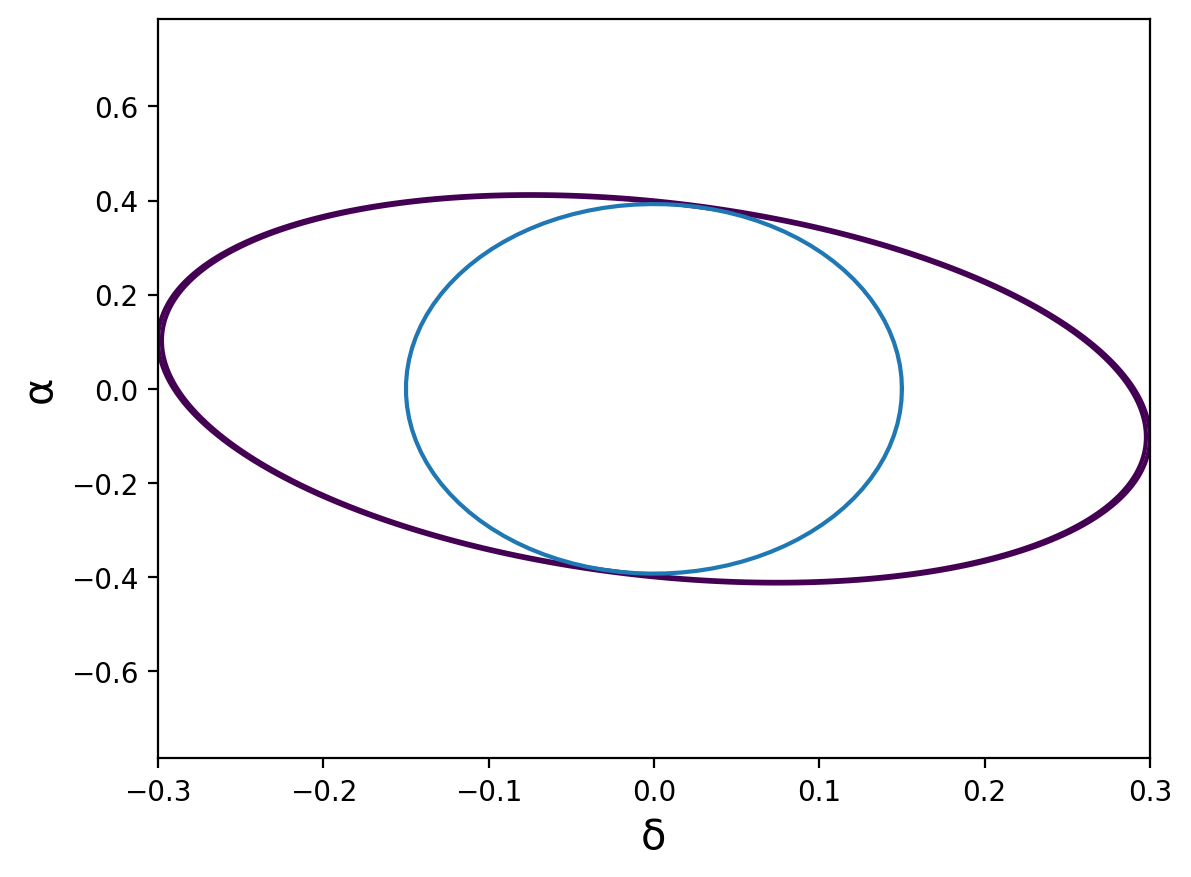
\includegraphics[width=0.8\textwidth]{figures/clf}
\caption{CLF computed using Algorithm~\ref{alg-find-clf}.
The purple lines (hardly distinguishable because superposed)
represent the $\mu$- and $\nu$-level sets of the CLF.
The blue line represents the boundary of $\calIreq$.}
\label{fig-clf}
\end{figure}

Finally, we use the CLF for the control of a car with
$v=1~\mathrm{m}/\mathrm{s}$.
By Theorem~\ref{thm-straight-curved}, the maximal allowed curvature satisfies
$\kappa_\maxtxt=1.49~\mathrm{m}^{-1}$ (corresponding to a radius of curvature of $R_\mintxt=0.66~\mathrm{m}$).
The path to follow is depicted in Figure~\ref{fig-path-following}
and consists in $N=250$ waypoints.
The choice of the control input is made in the same way as in the CoRL paper,
by minimizing the value of the CLF.
We see on Figure~\ref{fig-path-following} that the trajectory of the system
converges toward the path and never exit some safe region around this path.

\begin{figure}[h]
\centering
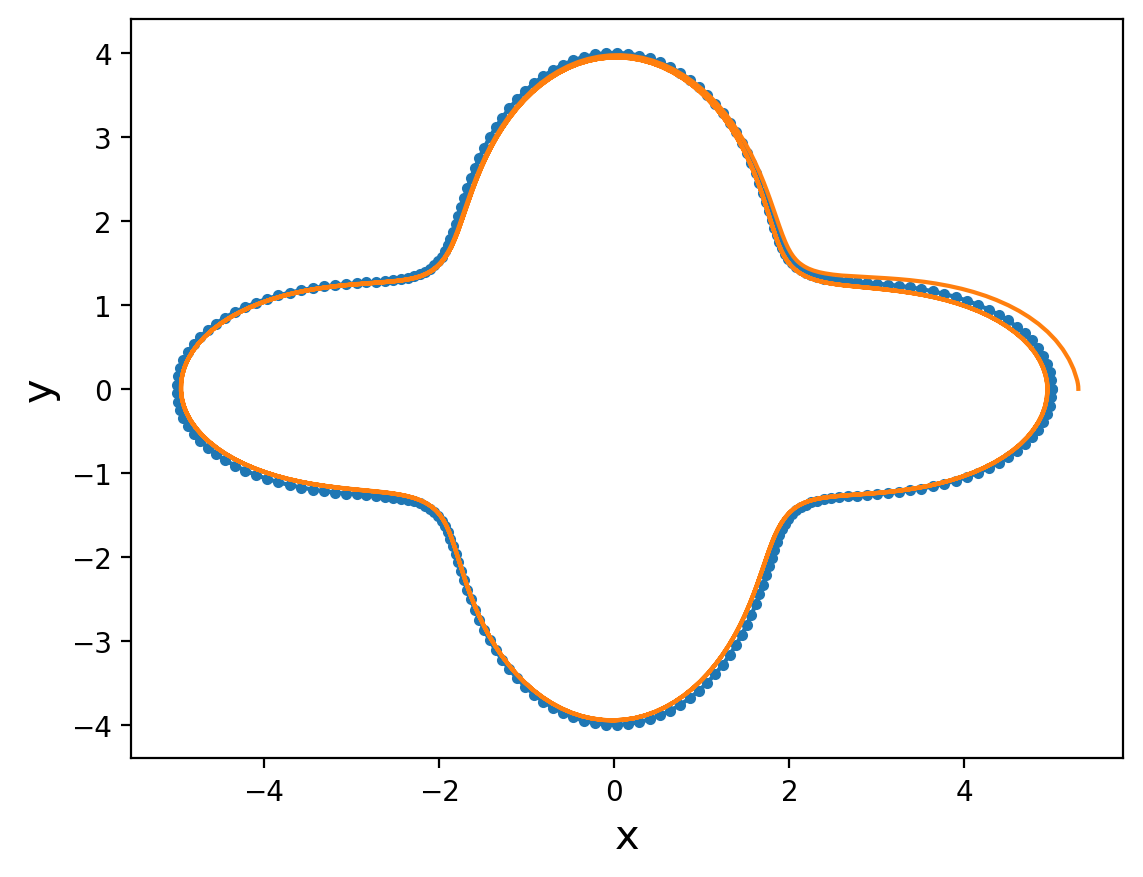
\includegraphics[width=0.8\textwidth]{figures/simupath}
\caption{The blue line represents the path to follow with
dots indicating the waypoints.
The orange line represents the system's trajectory.}
\label{fig-path-following}
\end{figure}

\end{document}